\documentclass[11pt,a4paper]{article}
\usepackage[T1]{fontenc}
\usepackage[utf8]{inputenc}
\usepackage[french]{babel}
\usepackage[left=2cm,right=2cm,top=2cm,bottom=2cm]{geometry}
\usepackage{amsmath}
\usepackage{amsfonts}
\usepackage{amssymb}
\usepackage{amsthm}
\usepackage{stmaryrd}
\usepackage{graphicx}
\usepackage{booktabs}
\usepackage{bbold}
\usepackage{minted}
\usepackage{colortbl}
\usepackage{multirow}
\usepackage[tikz]{bclogo}
\usepackage{xcolor}
\usepackage{hyperref}
\usepackage{diagbox}

\author{Mannequin Jeanne}
\date{01/10/2024}
\begin{document}
\begin{titlepage}

\newcommand{\HRule}{\rule{\linewidth}{0.5mm}}
\center 


\begin{figure}
    \centering
    
\includegraphics[width=0.5\linewidth]{\images\ssd_logo_couleur_noir-300x103.png}
\end{figure}



\textsc{\Large Master 2 Statistiques et Sciences des Données -BioStats}\\[1cm] % Major heading such as course name
\HRule \\[0.4cm]
{ \huge \bfseries Compte Rendu TP3 \\ Support Vector Machine (SVM)}\\[0.4cm]
\HRule \\[1.5cm]
\vspace{10cm}
\begin{center}
\begin{Large}
MANNEQUIN Jeanne \\
\end{Large}
\end{center}
    

\begin{center}
\vfill{
\includegraphics[width=0.1\linewidth]{\images\MONTPELLIER.jpg}\vspace{0.5cm}\\
\begin{Large} Année 2024 - 2025 \\
\end{Large}}



\end{center}

\end{titlepage}

\pagebreak

\tableofcontents
\pagebreak

\section*{Introduction}
Les \textbf{SVM} sont des algorithmes d'apprentissage supervisé servant à trouver une frontière de décision optimale entre plusieurs classes. Ils s'utilisent notamment dans les espaces de grande dimension. Leur objectif principal pour obtenir la meilleure prédiction est de maximiser la distance (ou la marge) entre chaque point et l'hyperplan. \\
Dans ce TP nous allons mettre en pratique ce type de techniques de classification sur données réelles et simulées au moyen du package \texttt{scikit\_learn} (lequel met en œuvre la librairie en C \texttt{libsvm}) et d’apprendre à contrôler les paramètres garantissant leur flexibilité (hyper-paramètres, noyau).\\

\section*{Premiers pas}
\addcontentsline{toc}{section}{Premiers pas}
\subsection*{Question 1}
\addcontentsline{toc}{subsection}{Question 1}
Le fichier \texttt{script.py} nous donne un exemple de classification avec la fonction \texttt{SVM} dont nous nous servons pour classifier la classe 1 contre la classe 2 du data set \texttt{iris} (ses deux premières variables) en utilisant un noyau linéaire.\\
On découpe le jeu de données en 2 sous-ensembles : un ensemble d'apprentissage et un ensemble de test. On laisse donc la moitié du jeu de données de côté pour l'évaluation.\\
On charge \texttt{iris} et des échantillons X et y une première fois et ces échantillons seront utilisés jusqu'à la fin du TP. Pour d'autres échantillons on obtient des résultats différents.
\begin{minted}[bgcolor=blue!07]{R}
# load the iris dataset
iris = datasets.load_iris()
X = iris.data
X = scaler.fit_transform(X)
y = iris.target
X = X[y != 0, :2]
y = y[y != 0]
\end{minted}
Ensuite on crée et entraîne le classifieur \texttt{SVM} avec le noyau linéaire. Puis on en sort les meilleur paramètres et son score pour évaluer la performance du modèle.
\begin{minted}[bgcolor=blue!07]{R}
# fit the model
parameters = {'kernel': ['linear'], 'C': list(np.logspace(-3, 3, 200))}
clf_linear = GridSearchCV(SVC(), parameters, n_jobs=-1)
clf_linear.fit(X_train, y_train)

print("Meilleurs paramètres pour le noyau linéaire : ", clf_linear.best_params_)

# compute the score
train_score = clf_linear.score(X_train, y_train)
test_score = clf_linear.score(X_test, y_test)

print('Generalization score for linear kernel: %s, %s' % (train_score, test_score))
\end{minted}
On trouve par exemple ici une valeur de $C$ d'environ 0.042 . $C$ est plutôt faible, ce qui veut dire que le modèle accepte plus d'erreurs de classification pour permettre une marge plus large. Cela donnera une frontière plus lisse mais risquerais de faire du sous-apprentissage (en opposition au sur-apprentissage) en cas jeux de données à peu de valeurs (ce n'est pas le cas ici).\\
On trouve également 0.78 et 0.68 comme meilleures scores pour respectivement l'échantillon d'entraînement et celui de test. Ces scores semblent bon sans être excellents. On constate une perte de 0.1 entre l'échantillon d'entraînement et celui de test, ce qui indique une potentielle baisse de performance sur les valeurs non étudiées. Cela peut également indiquer un overfitting.\\
Le score de l'échantillon d'entraînement a beau être bon, la différence avec le score de test indique que le modèle, avec ces échantillons initiaux, pourrait faire mieux avec d'autres paramètres. 

\subsection*{Question 2}
\addcontentsline{toc}{subsection}{Question 2}
Essayons donc par exemple d'effectuer le même schéma avec un noyau différent, le noyau polynomial, et comparer de les scores obtenus.
\begin{table}[H]
    \centering
    \begin{tabular}{|c|c|c|c|}
        \hline
        & train\_score & test\_score & Différence \\ 
        \hline
        Noyau linéaire & 0.78 & 0.68 & 0.1 \\
        \hline
        Noyau polynomial & 0.76 & 0.7 & 0.06 \\
        \hline
    \end{tabular}
    \caption{Scores pour les noyaux linéaire et polynomial}
    \label{Tableau 1}
\end{table}
Dans le tableau~\ref{Tableau 1} on voit que les scores avec le noyau polynomial sont globalement meilleurs, car même si le score de l'échantillon d'apprentissage est plus bas, la différence avec celui de test est encore plus basse, donc pas ou peu d'overfitting !

\section*{SVM GUI (optionnel)}
\addcontentsline{toc}{section}{SVM GUI (optionnel)}
\subsection*{Question 3 (bonus)}
\addcontentsline{toc}{subsection}{Question 3 (bonus)}
On fait tourner le code disponible sur le fichier 
En augmentant le paramètre $C$ la marge se réduit et inversement en diminuant C.

\section*{Classification de visages}
\addcontentsline{toc}{section}{Classification de visages}
Dans cette partie, on s'intéresse à la classification de visage. On va donner au modèle des images d'un certain Tony Blair puis on va lui demander de différencier cette personne d'une autre : Colin Powell. Voici en figure~\ref{blair} les photos données au modèle :
\begin{figure}[H]
    \centering
    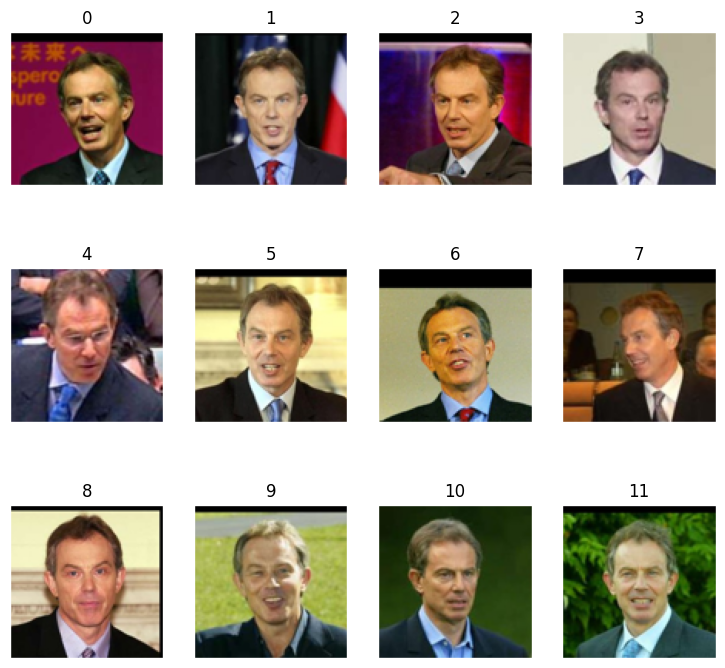
\includegraphics[width=0.5\linewidth]{\images\tony_blair.png}
    \caption{Photos de Tony Blair données au modèle pour entraînement}
    \label{blair}
\end{figure}
On regarde ensuite les résultats avec l'échantillon de validation sur la figure~\ref{blair_or_powell}: \\
\begin{figure}[H]
    \centering
    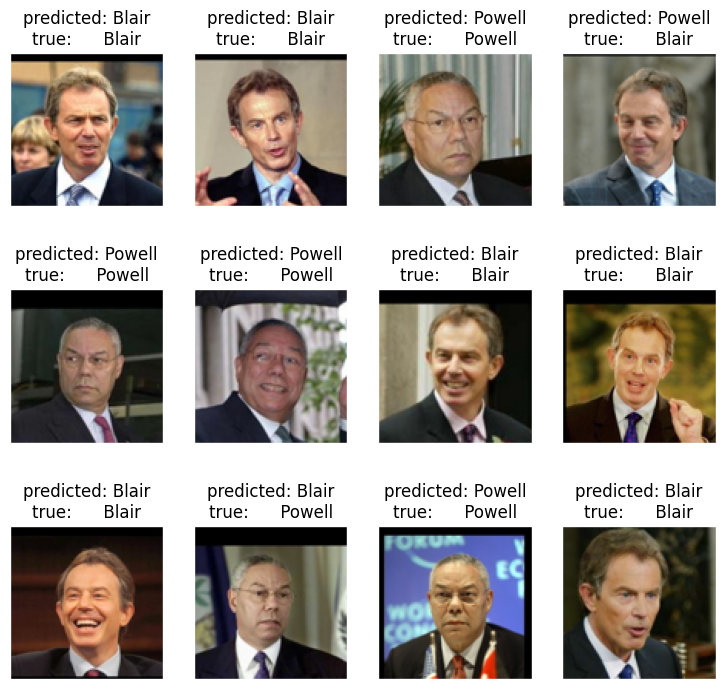
\includegraphics[width=0.5\linewidth]{\images\blair_or_powell.png}
    \caption{Résultat des prédictions du modèle SVM par image de Blair et de Powell}
    \label{blair_or_powell}
\end{figure}
Le "chance level", c'est-à-dire la précision que le modèle atteindrait s'il prédisait toujours la classe majoritaire, est ici d'environ 0.62 . C'est la valeur à laquelle on va comparer l'"accuracy" du modèle. L'"accuracy" est, elle, d'environ 0.92 . Le résultat est bon, mais quels sont les paramètres choisis ?

\subsection*{Question 4}
\addcontentsline{toc}{subsection}{Question 4}
En premier lieu, on se propose d'étudier le score d'apprentissage selon C choisi entre $10^{-5}$ et $10^{5}$. Comme on le voit sur cette figure~\ref{scores-selon-C} : le score augmente très rapidement jusqu'à atteindre son maximum d'environ 0.92 à 0.001=$10^{-3}$ (c'est le score que l'on avait trouvé pour la classification de visage en explication de cette partie), puis baisse très légèrement à environ 0.91 jusqu'à $10^{-2}$ et stagne jusqu'à la fin. On aura donc tendance à choisir un $C$ valant 0.001 pour cet échantillon, c'est ce que le modèle fait automatiquement.
\begin{figure}[H]
    \centering
    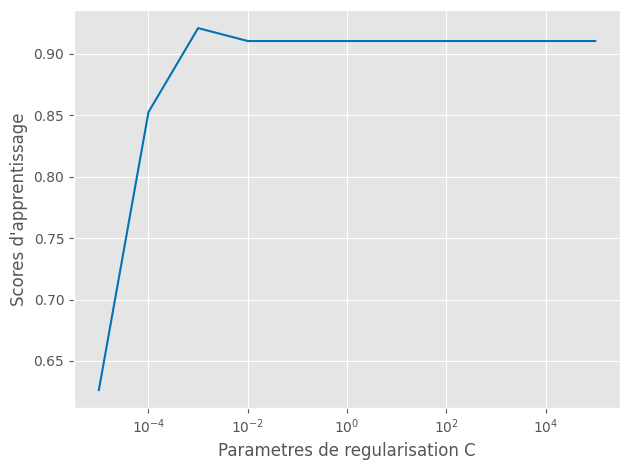
\includegraphics[width=0.6\linewidth]{\images\scores d'apprentissage selon C.png}
    \caption{Scores d'apprentissage selon C}
    \label{scores-selon-C}
\end{figure}

\subsection*{Question 5}
\addcontentsline{toc}{subsection}{Question 5}
Intéressons nous maintenant au score de notre modèle si on ajoute du bruit. Logiquement, le score devrait chuter. On lance donc le code suivant sur nos données :
\begin{minted}[bgcolor=blue!07]{R}
    n_features = X.shape[1]
    # On rajoute des variables de nuisances
    sigma = 1
    noise = sigma * np.random.randn(n_samples, 300, )
    X_noisy = np.concatenate((X, noise), axis=1)
    X_noisy = X_noisy[np.random.permutation(X.shape[0])]
\end{minted}
On applique ensuite le modèle \texttt{SVM} sur les données sans nuisances puis avec nuisance pour comparer les scores. On obtient les résultats suivants (arrondis à $10^{-2})$ :
\begin{table}[H]
    \centering
    \begin{tabular}{|c|c|c|c|}
        \hline
        & train\_score & test\_score & Différence \\ 
        \hline
        Sans variable de nuisance & 1.00 & 0.92 & 0.08 \\
        \hline
        Avec variable de nuisance & 0.99 & 0.57 & 0.42 \\
        \hline
    \end{tabular}
    \caption{Scores sans et avec variable de nuisance}
    \label{Scores bruit}
\end{table}
On constate que le score d'apprentissage ne s'en trouve que très peu diminué mais que l'écart avec le score de validation a drastiquement augmenté. Cette conclusion semble logique, en ajoutant du bruit, le modèle se construit sur des choses "fausses", potentiellement éloignés du réel modèle et donc diminuant le score de validation.\\

\subsection*{Question 6}
\addcontentsline{toc}{subsection}{Question 6}
Tentons enfin d'améliorer la prédiction du modèle en réduisant la dimension. On fait tourner le code suivant pour 5, 10, 15, 20, 25, 80, 120, et 200 composantes : 
\begin{minted}[bgcolor=blue!07]{R}
n_components = 120  # On joue avec ce parametre
pca = PCA(n_components=n_components).fit(X_noisy)
X_reduced = pca.fit_transform(X_noisy)
\end{minted}
Le code étant très longs à tourner (plus de 10h pour ces 8 valeurs différentes), les scores pour 5, 10, 15, 20, et 25 composantes nous ont gracieusement été donnés par Monsieur FESTOR Quentin, collègue de travail avec un ordinateur puissant et la patience qui nous a manqué. Pour 80, 120 et 200 composantes le code tournait beaucoup plus rapidement. Nous nous permettrons également d'ajouter la variance expliquée pour chaque nombre de composantes. On obtient le tableau suivant (arrondis à $10^{-2}$):
\begin{table}[H]
    \centering
    \begin{tabular}{|c|c|c|c|c|}
        \hline
        \diagbox{Nb de composantes}{Échantillons}& train\_score & test\_score & Différence & Variance expliquée \\ 
        \hline
        5 & 0.61 & 0.62 & 0.01 & 0.44 \\
        \hline
        10 & 0.61 & 0.64 & 0.03 & 0.57 \\
        \hline
        15 & 0.65 & 0.59 & 0.06 & 0.63 \\
        \hline
        20 & 0.66 & 0.59 & 0.07 & 0.68 \\
        \hline
        25 & 0.69 & 0.58 & 0.11 & 0.71 \\
        \hline
        80 & 0.83 & 0.58 & 0.25 & 0.87 \\
        \hline
        120 & 0.88 & 0.55 & 0.33 & 0.90 \\
        \hline
        200 &  &  &  &  \\
        \hline
    \end{tabular}
    \caption{Scores pour les noyaux linéaire et polynomial}
    \label{Scores composantes}
\end{table}
On observe qu'en diminuant la dimension, on diminue le score de l'échantillon d'apprentissage. En revanche, ce qui est intéressant ici c'est que l'écart avec le test de validation s'en trouve bien diminué également ! Le modèle est donc plus fiable ! Pour ce qui est de la variance explique, elle augmente bien évidemment en augmentant le nombre de composantes. On trouve une variance expliquée de 0.44 pour une dimension de 5 composantes, ce qui est assez faible. En revanche, en prenant par exemple 25 composantes, on arrive à un score sur l'échantillon d'apprentissage de 0.69 (reste acceptable), avec une différence à l'échantillon de test autour de 0.1 (acceptable également) et une variance expliquée de 0.71 (relativement correct).\\
En conclusion, le nombre de composantes choisi dépendra du résultat désiré : plus bas si on accepte de perdre de l'information, plus haut si on accepte un modèle moins performant. On cherche à maximiser les scores et la variance expliquée, tout en minimisant l'écart entre les score d'apprentissage et de validation. Ici, 25 composantes me semble être un bon compromis.

\section*{Conclusion}
Ce TP a permis de mettre en pratique les concepts de $SVM$ sur des données réelles et simulées, en explorant l’impact des paramètres sur les performances. Les résultats montrent que le choix du noyau et des paramètres tels que $C$ influencent directement la capacité du modèle, comme observé dans les comparaisons entre noyau linéaire et polynomial. En ajoutant du bruit et en réduisant la dimension des données, nous avons constaté que l’ajustement du modèle est essentiel pour éviter le sur-apprentissage, tout en maximisant les scores d’apprentissage et de validation.

\end{document}
